%
% file : learn_git.tex
% date : jeudi 19 décembre 2019, 13:19:09 (UTC+0100)
% author : sedelpeuch
% description :
\documentclass[a4paper,10pt]{article}
\usepackage[utf8]{inputenc}
\usepackage[T1]{fontenc}
\usepackage[french]{babel}
\usepackage{graphicx}
\usepackage{float}
\usepackage{amsmath}
\usepackage{amssymb}
\usepackage{mathrsfs}
\usepackage{color}
\usepackage{fancyhdr}
\usepackage{pdfpages}
\usepackage{layout}
\usepackage{multicol}
\usepackage{setspace}
\usepackage{csvsimple}
\usepackage[table]{xcolor}
\usepackage[colorlinks=true]{hyperref}
\usepackage{tikz, tkz-tab}
\usepackage[top=2cm,bottom=2cm,left=2cm,right=2cm]{geometry}
\usepackage{amsthm}
\usepackage{listings}
\usepackage{verbatim}
\usepackage{transparent}
\usepackage{eso-pic,graphicx}

\AddToShipoutPicture*{
    \unitlength=0cm
    \put(0,0){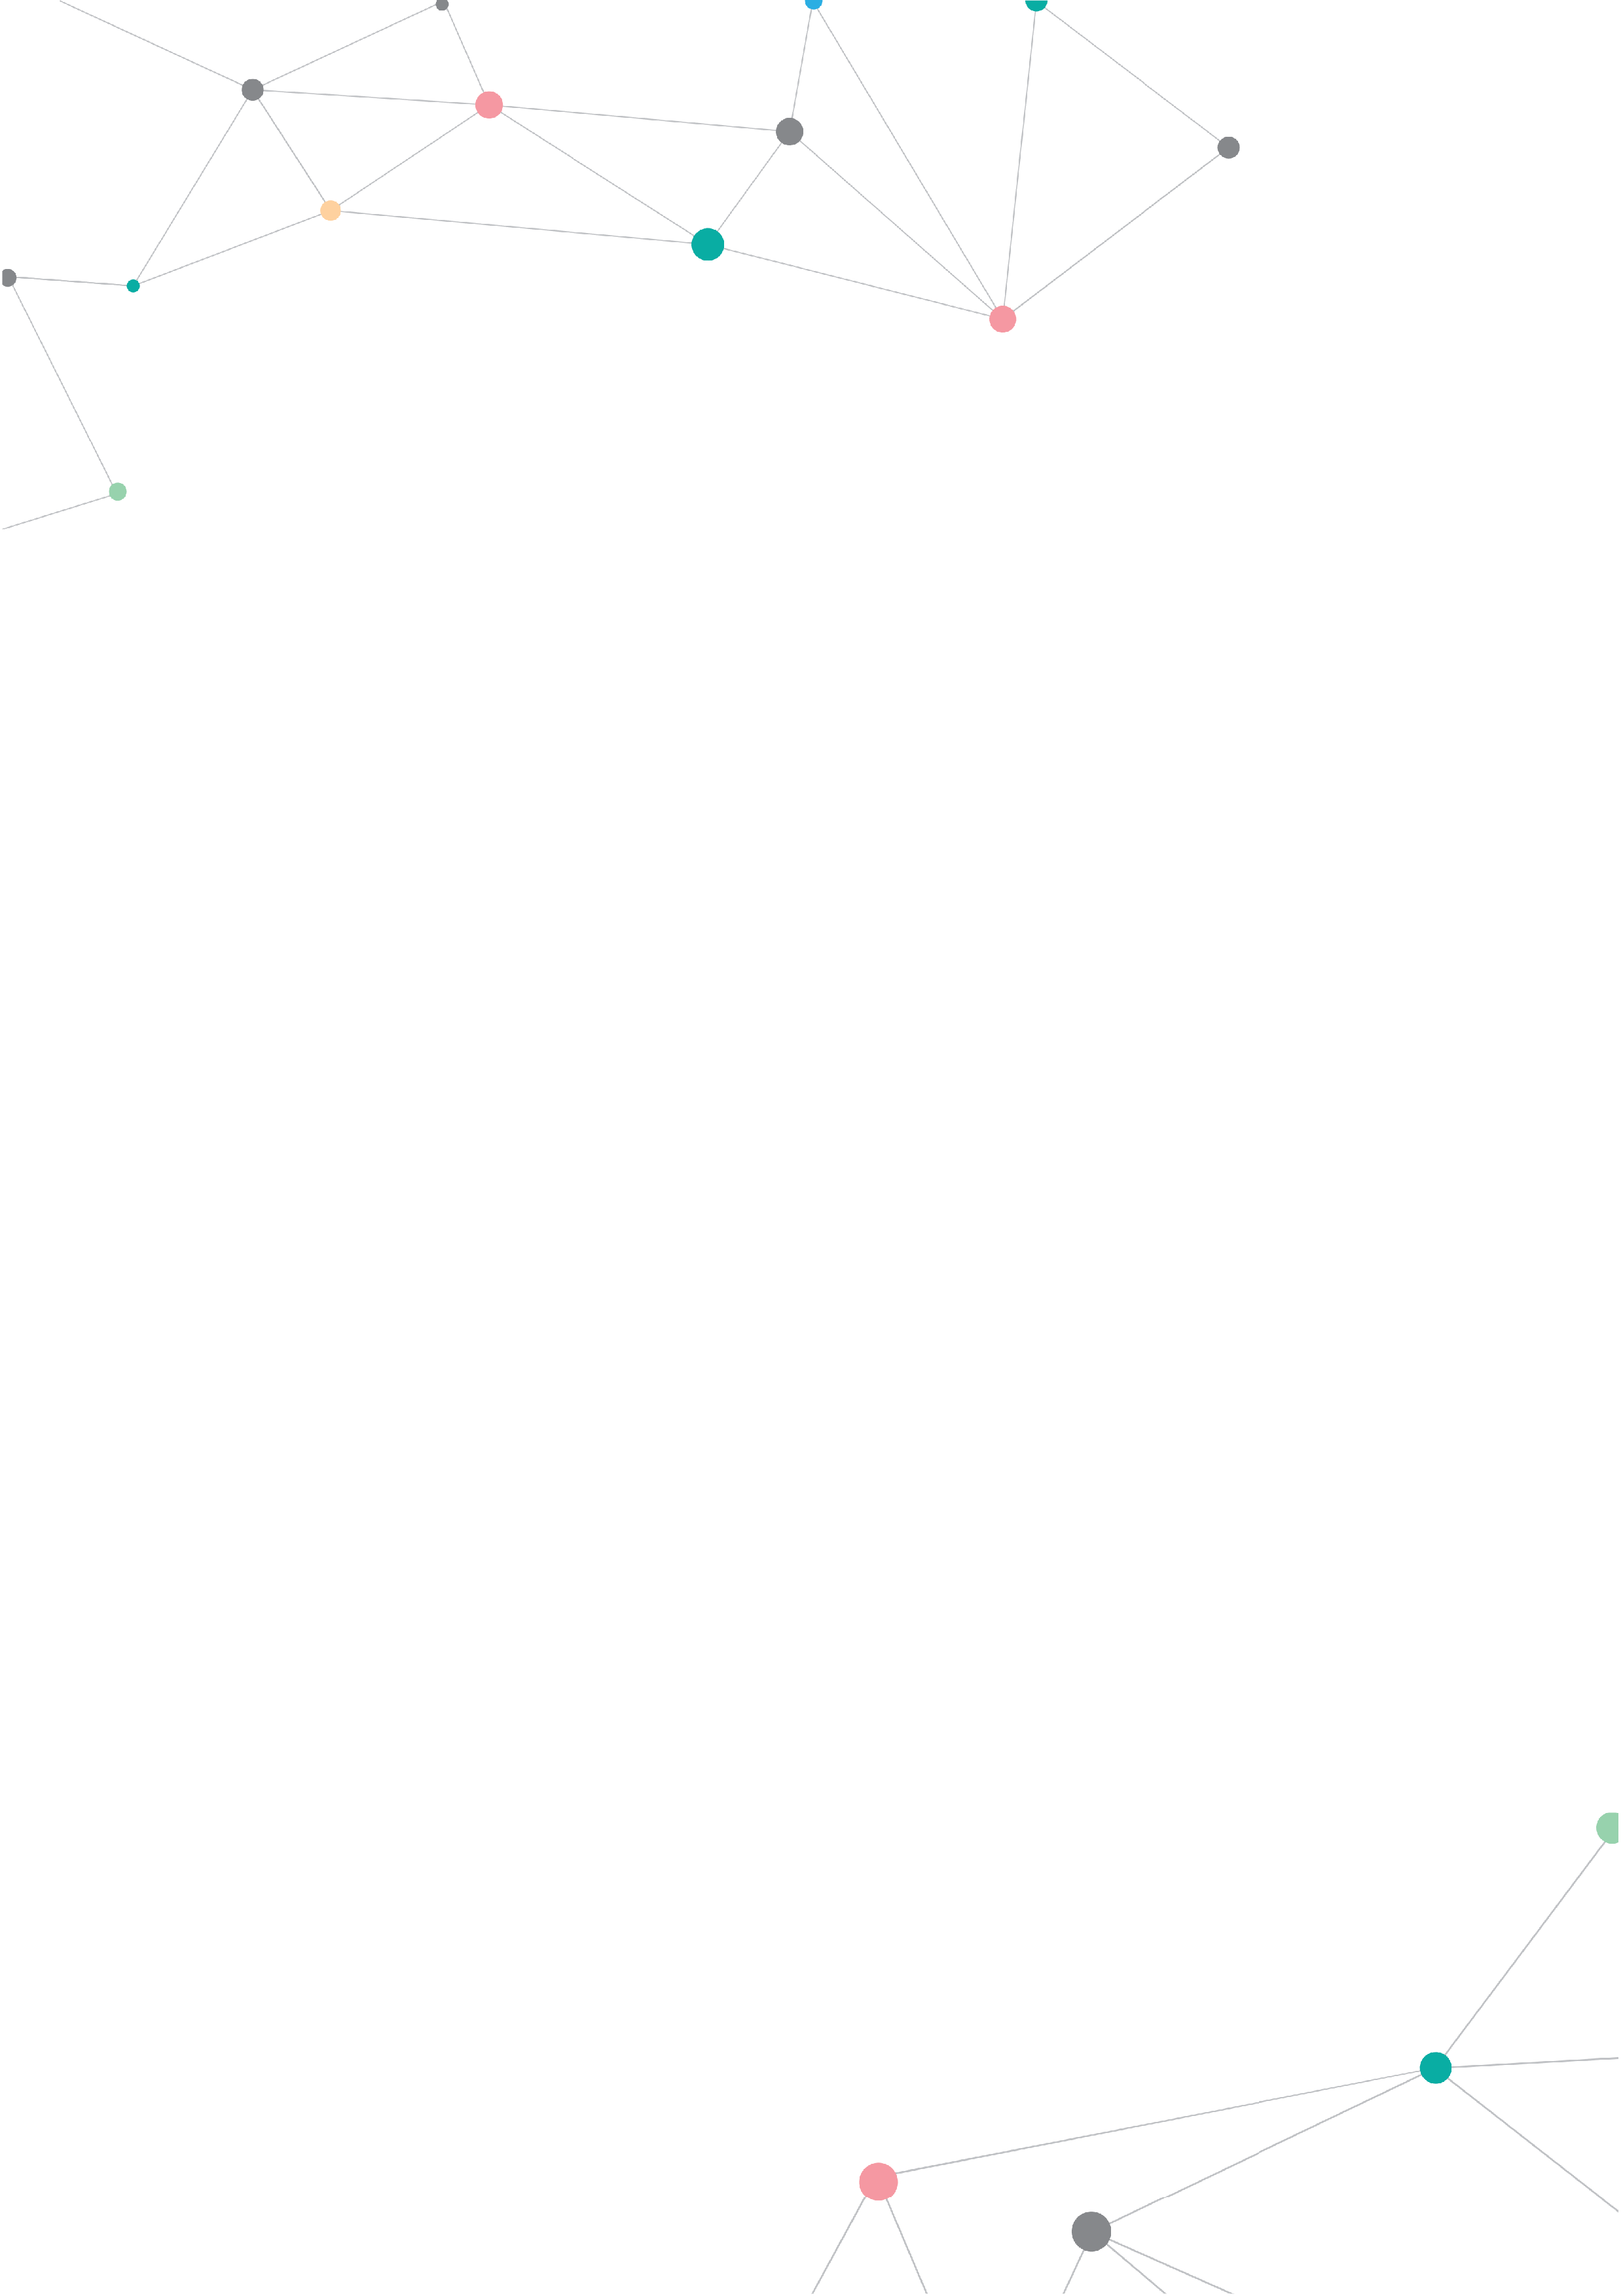
\includegraphics{filigramme3.png}}

}
\AddToShipoutPicture{%
  \unitlength=1cm
    \put(1.6,8){\transparent{0.3}
\includegraphics[width=18cm,
        height=13cm]{filigrame.png}}
  }

\setlength{\parindent}{0.785cm}
\setlength{\parskip}{1ex plus 0.5ex minus 0.2ex}
\newcommand{\hsp}{\hspace{20pt}}
\newcommand{\HRule}{\rule{\linewidth}{0.1mm}}
\newcommand{\therule}{\rule{5cm}{0.05mm}}


\usepackage{xcolor}
\begin{document}
\begin{spacing}{1.5}
\graphicspath{{image/}}
  \begin{titlepage}
\begin{sffamily}
\begin{center}
  \vspace*{\stretch{1}}
\textbf{\textsc{\LARGE Eirbot \\ Association de robotique de
    l'ENSEIRB-MATMECA}}\\[0.5cm]
\HRule \\[0.2cm]
       {\Huge \bfseries Présentation des projets 2020 \\
       \HRule \\[0.5cm]

\vspace*{\stretch{1}}
       
\includegraphics[scale=0.5]{LogoEirbot.png}
       \vfill}
  \end{center}
  \end{sffamily}
\end{titlepage}
\setcounter{tocdepth}{2}
\newpage
\pagestyle{fancy}
\lhead{}
\chead{\textbf{Présentation des projets 2020}}
\rhead{\thepage}
\lfoot{}
\cfoot{}
%% \section{Qui sommes nous ?}
%% Association de robotique de l'ENSEIRB-MATMECA crée en 2003, Eirbot est avant
%% tout un groupe de passionné d'électronique, d'informatique et de mécanique.
%% Chaque année, Eirbot acceuille un certain nombre d'élève ingénieur de première,
%% deuxième et troisième année. Cette année l'association contient une trentaine de membre
%% actifs. \\
%% Forte d'une équipe motivée, diversifiée, stimulée et soudée nous nous réunissons
%% autour d'un projet commun : la coupe de france de robotique. \\
%% Eirbot participe depuis sa création en tant que club (en 1997) à la coupe de
%% France de robotique
%% Les objectifs de l'association sont les suivants
%% \begin{itemize}
%% \item Participation à la coupe de France de robotique à la Roche sur Yon tous
%% les ans
%% \item Formations des éléves à la création d'un robot de A à Z (design/routage
%% de cartes électroniques, design de pièces 3D et impression 3D, initiation aux
%% systèmes embarqués)
%% \item Participation aux robots Maker's Day et autres évéenements organisés
%% dans l'école
%% \item transmission du savoir entre les anciens et les nouveaux adhérents
%% Nous disposons d'un local avec plusieurs outils mécanique et électroniques
%% (scies à chantourner, fer à souder, imprimante 3D, etc) situé dans l'enceinte
%% de l'école.
%% \end{itemize}
%% L'association est en partie financée par l'école et le reste par les
%% partenariats professionnels. Dans l'objectif de continuer nos activités au
%% mieux, nous sommes à la recherche de partenariats. Ce derniers peuvent être de
%% toutes formes.
%% \newpage
\section{Notre projet}
Cette année, Eirbot prend le large ! Nos robots doivent partir voguer à travers
le monde. Nous allons devoir maitriser la navigation pour arriver à bon port.
C'est après une tempête qu'il faudra reconstruire le chenal, réactiver le phare
et redresser les manches à air pour espérer gagner. Nos robots évolurons sur la
table suivante
\begin{figure}[H]
  \center
  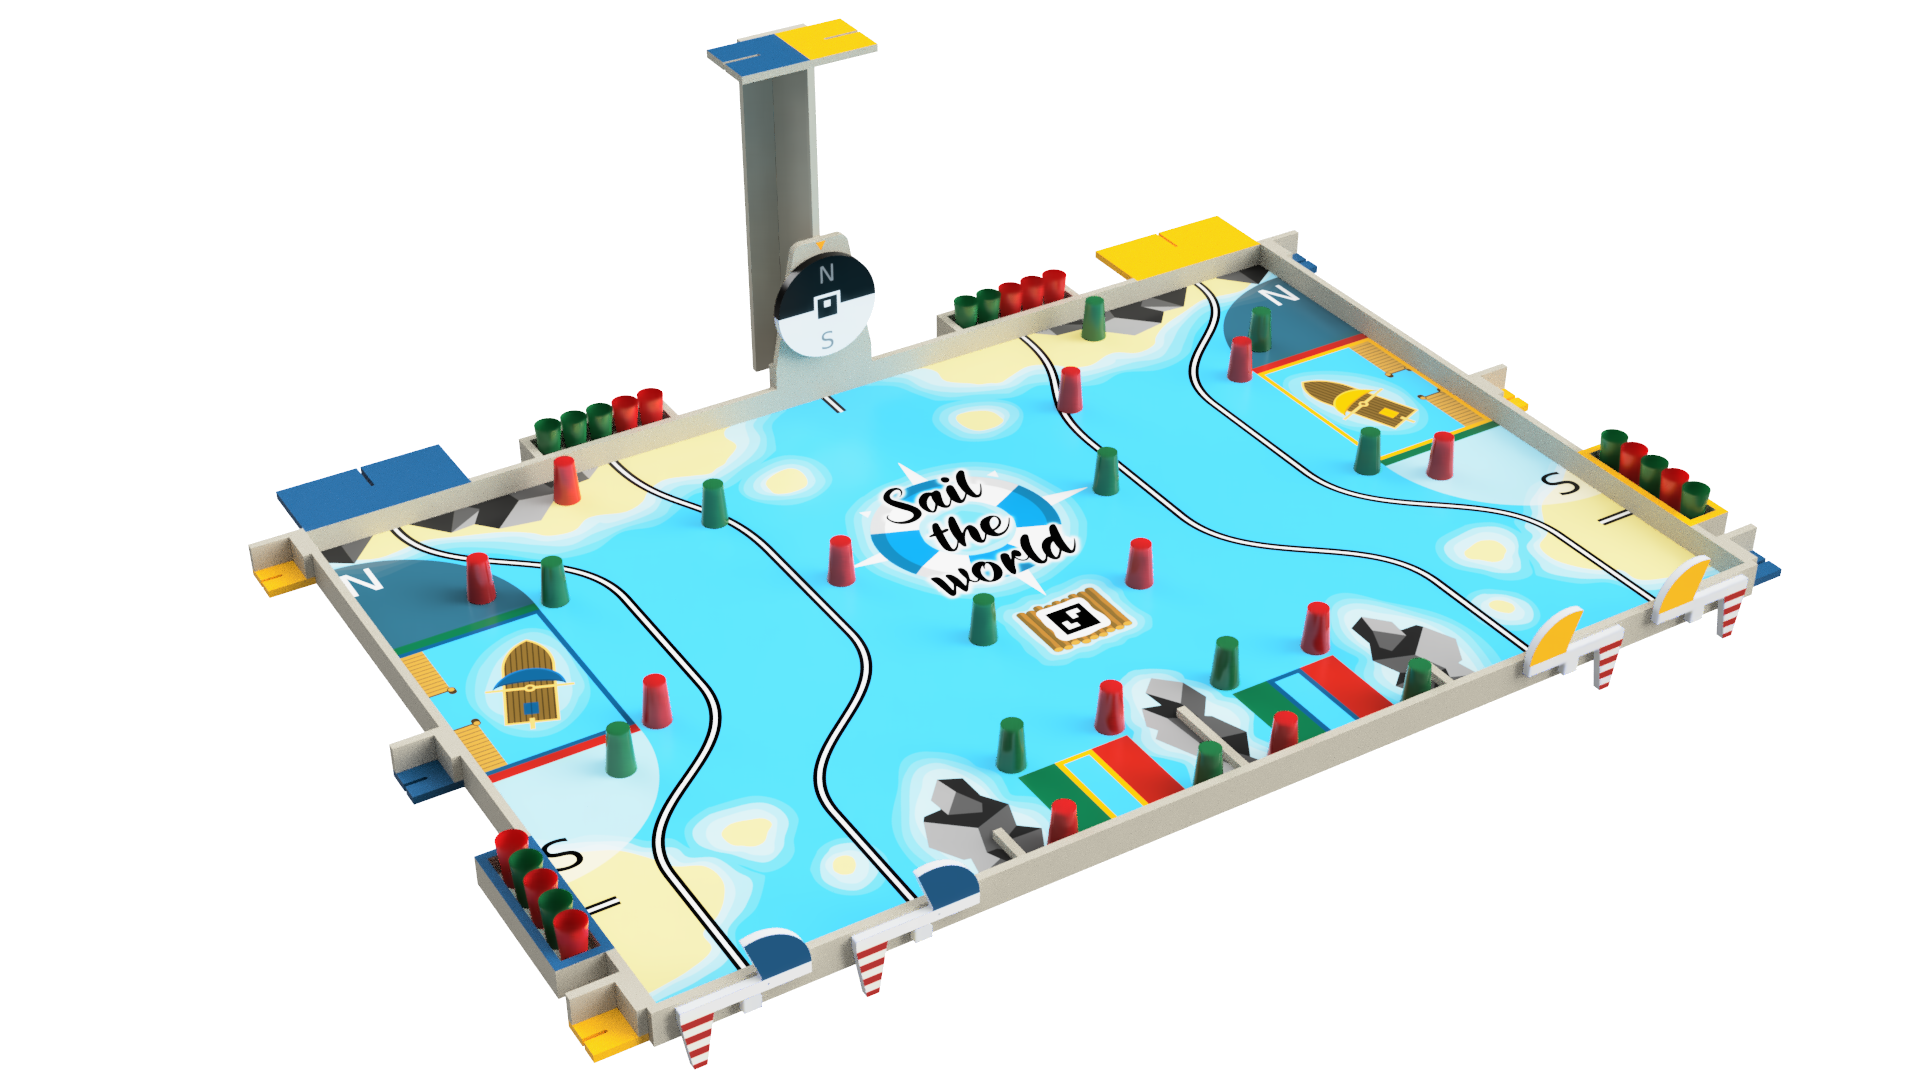
\includegraphics[scale=0.2]{table.png}
  \caption{Schéma de la table de jeu}
\end{figure}
En plus de l'environnement de jeu nous devons suivre des règles précises
disponibles sur ce \href{https://www.coupederobotique.fr/wp-content/uploads/Eurobot2020_Rules_Cup_OFFICIAL_FR.pdf}{lien}.
\subsection{Vue d'ensemble du projet et objectif de l'association}
Voyons tout d'abbord l'objectif que nous allons nous fixer pour ce projet. Nous
avons décidé en commun des différentes actions et des différentes tâches à
réaliser. Nous décidons de réaliser les actions suivantes, activer le phare,
redresser les deux manches à air, décoder la boussole et retourner à bon port.
Nous misons sur la qualité des actions et non sur la quantité de ces
dernières.

Nous avons ensuite découvert le processus de fabrication d'un robot, grâce
à l'aide des promotions supérieures nous comprenons qu'il y aura 4 grands
domaines :  la mécanique du robot (la structure, les actionneurs, le phare),
l'électronique (alimentation du robot,
contrôle des actionneurs, création du compteur de points etc), l'asservissement (direction
précise du robot) et la stratégie (recherche de chemin, choix des actions à
faire etc).
\subsection{Plans du robot}
Nous avons ensuite réalisé les plans de notre robot. Nous avons pu le rendre
concret en majeur partie grâce à la découpe laser du FabLab de l'ENSEIRB MATMECA
et à notre imprimante 3D. En addition nous utilisons des profilés pour monter la
structure et créer des étages facile à monter et démonter.
\begin{figure}[H]
  \center
  
\includegraphics[scale=0.3]{LogoEirbot.png}
  \caption{Photo de l'état actuel de notre robot}
\end{figure}
Concernant notre phare, il doit se deployer et réaliser un balayage lumineux (il
doit faire moins de 30 cm avant l'activation et plus de 70 cm après). Nous optons
pour imprimer grâce à notre imprimante 3D un bras robotique, le système
d'éclairage de notre phare sera similaire à celui d'un vrai phare. Voici
l'avancement actuel de notre phare
\begin{multicols}{2}
\begin{figure}[H]
  \center
  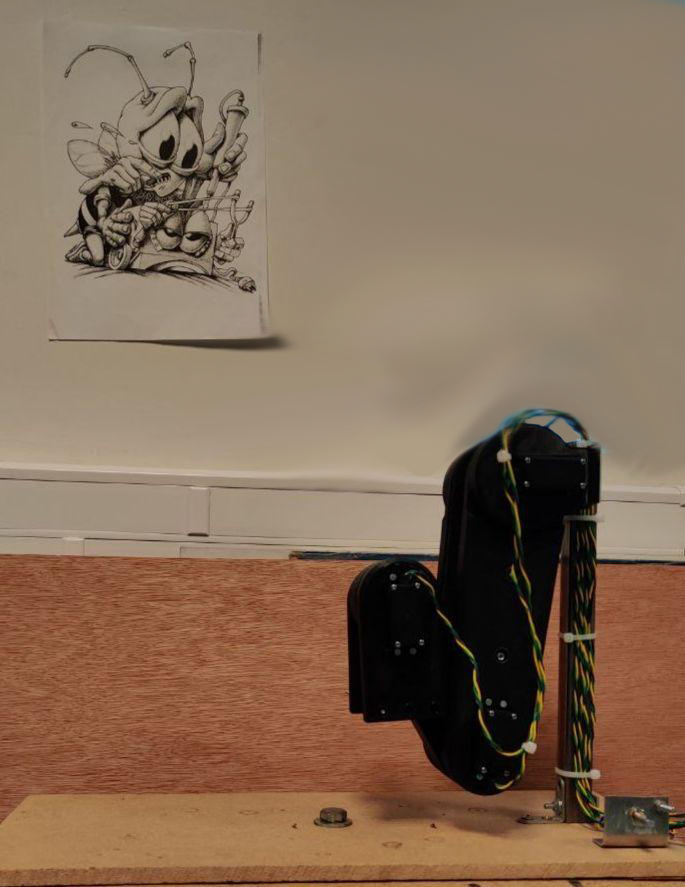
\includegraphics[scale=0.3, height=8cm]{phare_r.png}
  \caption{Photo de l'état actuel de notre phare replié}
\end{figure}
\columnbreak
\begin{figure}[H]
  \center
  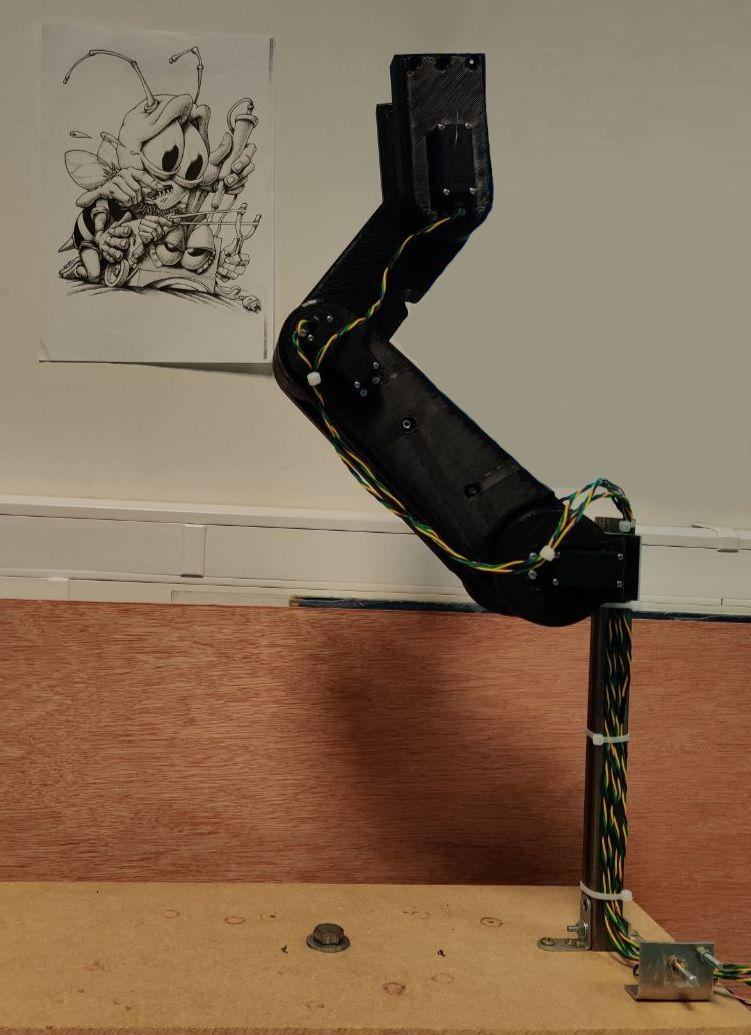
\includegraphics[scale=0.3, height=8cm]{phare_d.png}
  \caption{Photo de l'état actuel de notre phare déplié}
\end{figure}
\end{multicols}
\subsection{Fonctionnement général du robot}
Comme dit précédemment nous misons sur la qualité de nos actions plutôt que la
quantité. Nous divisons alors le travail informatique en deux parties. D'une
part l'Asservissement qui est implémenté sur une Nucléo-F429ZI. D'autre part, la
stratégie qui est implémentée sur une Raspberry pi 3b+. En addition nous avons du
créer un protocole de communication entre les deux cartes.\\

\subsubsection{Asservissement}
Nous pouvons commencer par décrire succinctement l'asservissement que nous avons
élaboré \\ %mettre paragraphe de clément si il existe

\subsubsection{Stratégie}
Nous pouvons maintenant décrire notre stratégie. La stratégie dépend de deux
facteurs principaux, notre capacité à naviguer sur la table et notre capacité à
détecter les adversaires et à réagir lorsque nous tombons face à l'un de.
\\ \indent Pour la navigation nous implémentons un algorithme de recherche de
chemin connu dérivé de l'algorithme de Dijikstra : l'algorithme A*. Nous
décrivons rapidement son fonctionnement dans le paragraphe suivant, une
animation expliquant le principe de ce dernier est disponible sur ce
\href{https://fr.wikipedia.org/wiki/Algorithme_A*#/media/Fichier:Astar_progress_animation.gif}{lien}.\\ \indent
Nous avons modélisé la table comme une grille chaque case faisant $1 cm \times 1
cm$. Ainsi nous avons pu renseigner la position de tous les obstacles fixes. A
partir de cela nous pouvons expliquer le fonctionnement de l'algorithme. l'A*
commence à un noeud choisi. Il applique à ce dernier un cout initial, il estime
ensuite la distance entre ce noeud et le but à atteindre. Le noeud est alors
ajouté à une liste d'attente prioritaire, appelée \textit{open list}. \\ \indent
Premièrement l'algorithme récupère le premier noeud de l'\textit{open list}. Si
elle est vide, il n'y a aucun chemin du noeud initial à celui d'arrivé,
l'algorithme est en erreur. Si le noeud est celui d'arrivé, l'algorithme va
reconstruire le chemin complet et renvoyer le résultat. Ensuite, si le noeud
n'est pas le noeud d'arrivée alors de nouveaux noeuds sont crées pour tous les
noeuds contigus admissibles . L'A* calcule ensuite son coût et le stocke avec le
noeud. Ce coût est calculé à partir de la somme du coût de son ancêtre et du
coût de l'opération pour atteindre ce nouveau noeud. En parallèle l'algorithme
conserve la liste des noeuds qui ont été vérifiés, c'est la \textit{closed
  list}. Si un noeud nouvellement produit est déjà dans cette liste avec un coût
égal ou inférieur, on ne fait rien. Après, l'évaluation de la distance du
nouveau noeud au noeud d'arrivée est ajoutée au coût pour former l'heuristique
du noeud. Ce noeud est alors ajouté à la liste d'attente prioritaire, à moins
qu'un noeud identique dans cette liste ne possède déjà une heuristique
inférieure ou égale. Une fois ces étapes effectuées pour chaque nouveau noeud
contigu, le noeud original pris de la file d'attente prioritaire est ajouté à la
liste des noeuds vérifiés. Le prochain noeud est alors retiré de la file
d'attente prioritaire et le processus recommence.

Les détails technique des notre implémentation sont disponibles sur notre
\href{https://github.com/eirbot/eirbot2020-1A/blob/master/code/rasp/src/navigation.cpp}{Github}.
A ce stade, notre algorithme est opérationnel et nous pouvons d'un point $x,y$
donné rejoindre n'importe quel point $x',y'$ en évitant les obstacles fixes.
Nous allons maintenant présenter notre stratégie concernant les obstacles
mobiles c'est à dire les adversaires.

Nous utilisons un système infrarouge (GP2) pour la détection, ces derniers sont
placés juste au dessus des gobelets disposés sur la table (les gobelets sont
considérés comme des obstacles fixes, nous ne voulons pas les détecter avec le
système infrarouge). Lorsque nous détectons un robot adverse, la stratégie prend
un branchement, récupère l'information sur la distance que nous fournit le
système infrarouge, ajoute un obstacle puis relance la navigation ce qui permet d'éviter l'obstacle.
A la fin du branchement l'obstacle est détruit. A ce stade nous pouvons avons un
système de détection nous permettant d'éviter les robots adverses en les
contournants.

Nous avons présentés nos principales stratégies, nous n'avons pas décrit tous
nos codes mais seulement les principaux. Les autres codes sont disponibles sur
notre dépot \href{https://github.com/eirbot/eirbot2020-1A}{Github}.

\subsubsection{Protocole de communication}
En choisissant de séparer nos codes sur deux cartes différentes, nous avons une
difficulté supplémentaire qui apparait. Il faut réaliser un protocole de
communication permettant d'envoyer des ordres de la carte maître (Raspberry
Pi) vers la carte esclave (Nucléo). Cette dernière répond aux commandes par une
action (déplacement, activation des actionneurs, ...) ou par des
informations sur l'état du robot (position, capteurs de distance, ...). Nous
avons choisi d'établir la communication via un port série et nous avons créé un
protocole spécifique aux besoins de notre projet. Le protocole implémente un
système de confirmation des commandes et supporte des timeout. Prenons un
exemple simple, lorsque nous lançons la Navigation sur la Raspberry pi, l'A* va
calculer les positions à rejoindre, au fur et à mesure que l'algorithme trouve
les positions, il envoie une requete de déplacement via le port série, attend la
réponse du protocole et si il n'y a pas de soucis envoie la prochaine instruction.

\subsection{Electronique du robot}
\subsubsection{Carte d'alimentation}

La conception d'une carte d'alimentation est un étape fondamentale lors de la
mise en oeuvre d'un projet d'électronique.Cette dernière assure l'alimentation
du circuit à une tension souhaitée.La stabilité du signal doit être également
maintenue malgré les pertubations liés au circuit.

Pour le robot, nous avons opté pour une carte comportant 3 rails
d'alimentations.

\begin{figure}[H]
  \center
  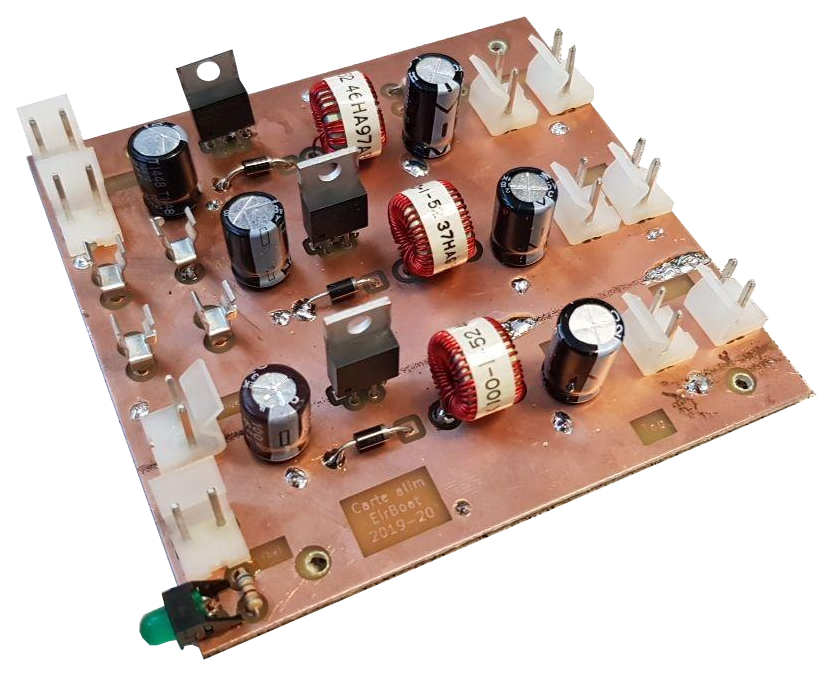
\includegraphics[scale=0.3]{carte.png}
  \caption{Etat actuel de notre carte d'alimentation}
\end{figure}

Deux de ces rails fournissent une alimentation de 5V,le premier alimente la
logique, le suivant les actionneurs. Le dernier est consacré aux moteurs,
alimenté en 12V.

\begin{figure}[H]
  \center
  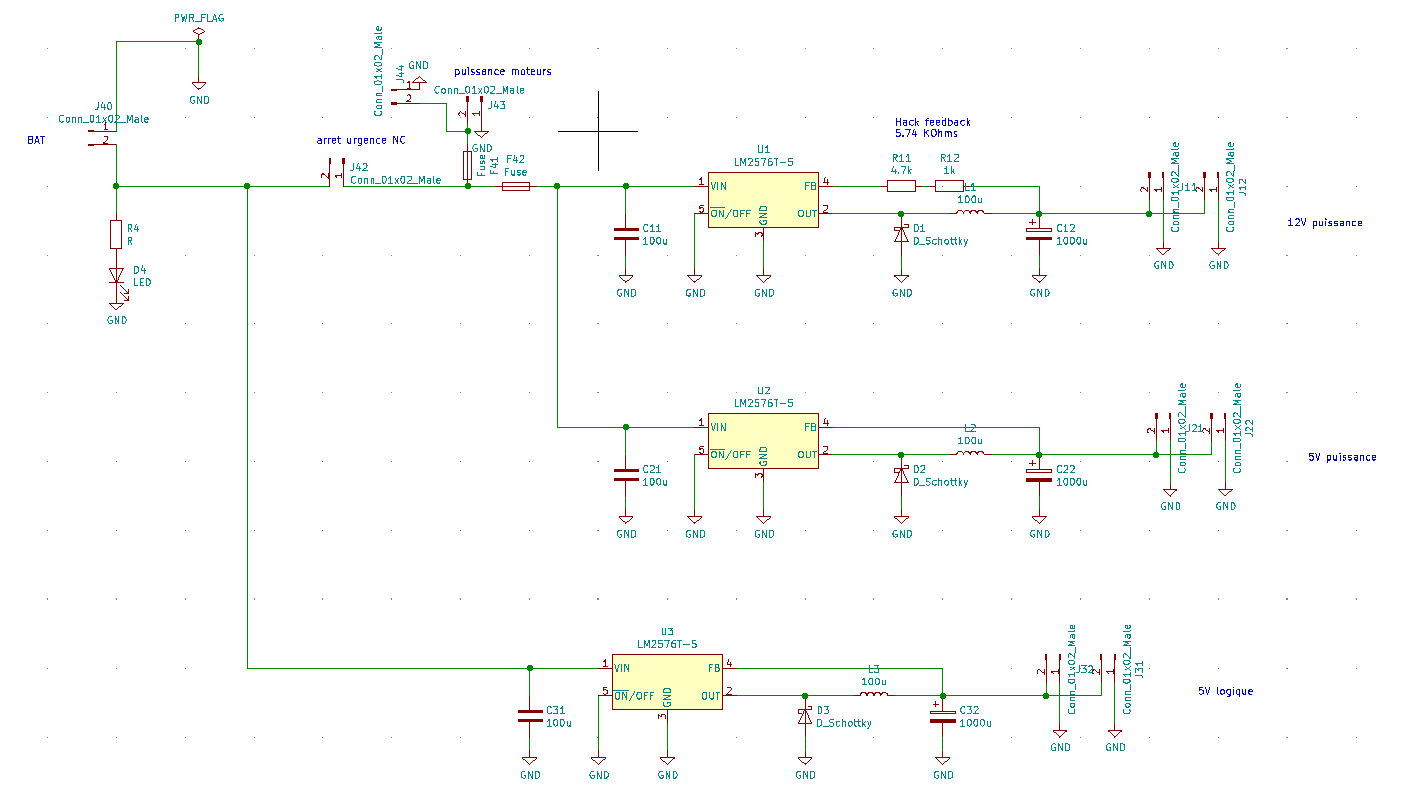
\includegraphics[scale=0.5]{schema.jpg}
  \caption{Schéma de conception de la carte}
\end{figure}

Chaque rail d'alimentation est structurée autour d'un buck. Un buck est une convertisseur de tension continue.Alimentation à découpage de la
micro-électronique, il possède un excellent rendement( 95 \% environ).

\begin{multicols}{2}
\begin{figure}[H]
  \center
  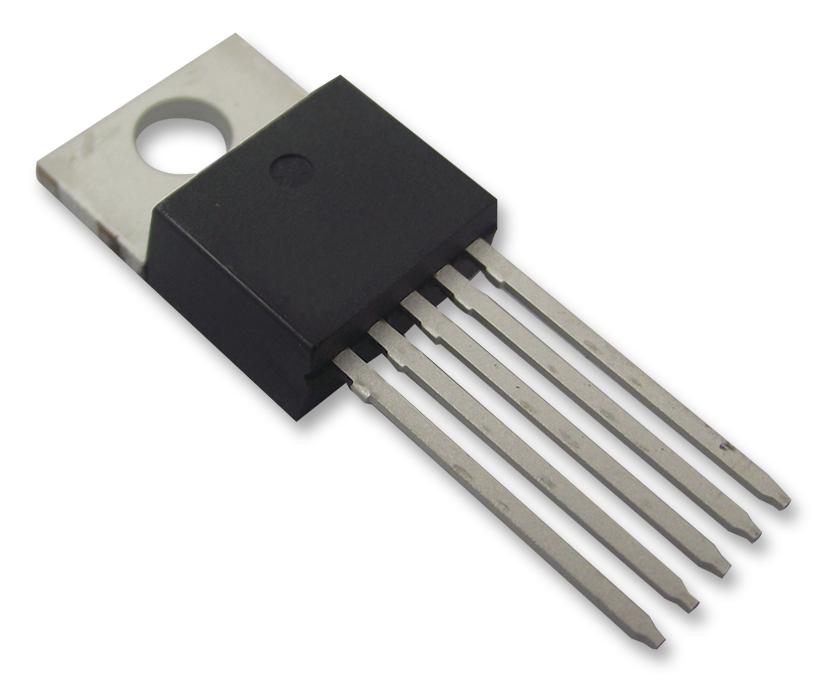
\includegraphics[scale=0.1]{buck.jpg}
  \caption{Image du composant électronique}
\end{figure}
\columnbreak
\begin{figure}[H]
  \center
  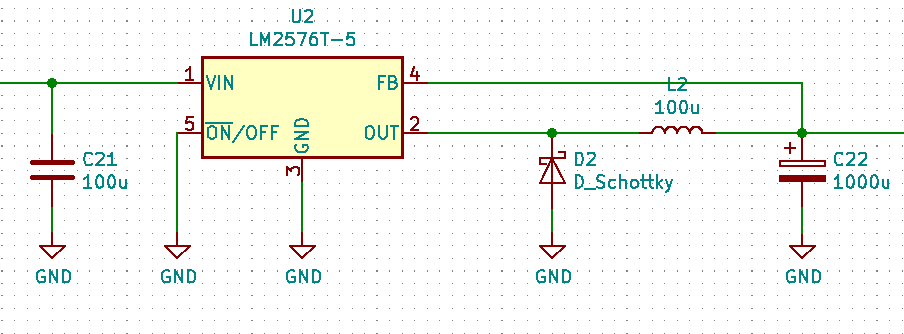
\includegraphics[scale=0.4]{buck.PNG}
  \caption{Schéma de conception d'un buck}
\end{figure}
\end{multicols}
Mis à part les composants, l'intégralité de la carte a été conçue par nos soins.
Le routage est une étape cruciale, elle consiste à relier les composants en
optimisant l'espace utilisé et en évitant les phénomènes perturbateurs. En
effet, la proximité physique des signaux peut provoquer,par exemple, des
phénomènes d'induction. L'intégralité de notre routage a été réalisé grâce au
logiciel kickad. On aboutit finalement à un calque du circuit. \\
Une fois que nous avons obtenu ce calque nous pouvons passer à la réalisation de
cette dernière grâce au matériel de l'ENSEIRB-MATMECA. Le perçage des trous et
la soudure des éléments se réalise avec le matériel de l'association.

\subsubsection{Carte de puissance}
En plus de l'alimentation du robot, nous
\newpage
\section{Projets antérieurs}
Notre association possède une certainne ancienté et en plus de participer à la
coupe de France nous réalisons plusieurs projets voici quelques photos des
projets et des robots des années précédentes
\begin{multicols}{2}
  \begin{figure}[H]
    \center
    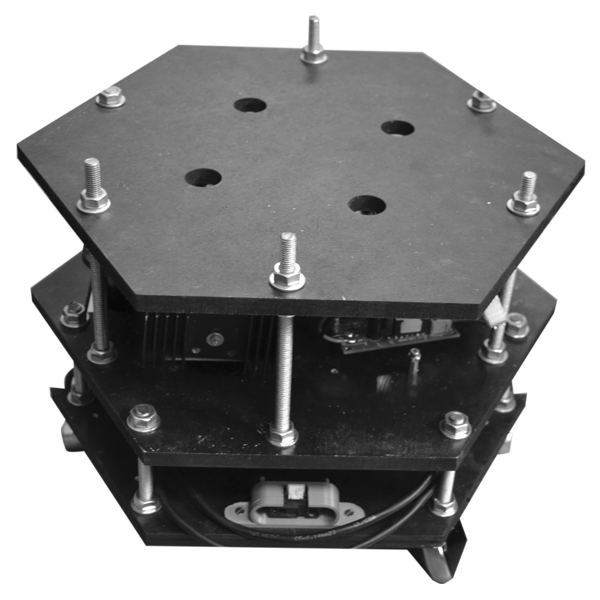
\includegraphics[scale=0.3]{1A2018.png}
  \end{figure}
  \columnbreak
  \begin{figure}[H]
    \center
    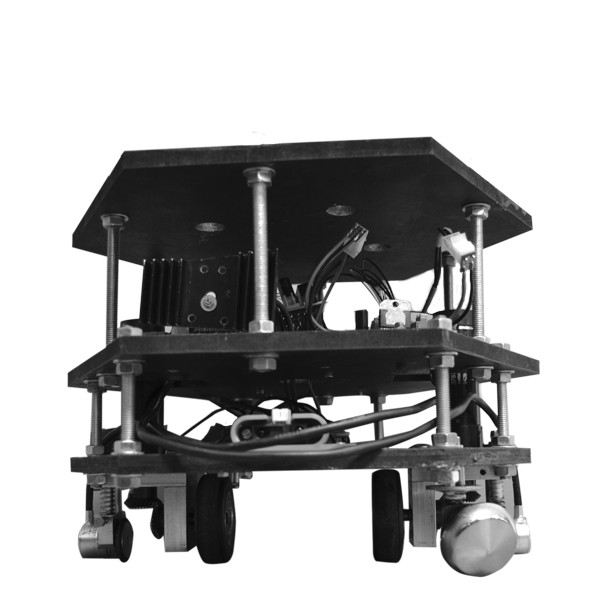
\includegraphics[scale=0.3]{1A2018(2).png}
  \end{figure}
\end{multicols}

\begin{multicols}{2}
  \begin{figure}[H]
    \center
    \includegraphics[scale=0.3]{2A2018.png}
  \end{figure}
  \columnbreak
  \begin{figure}[H]
    \center
    \includegraphics[scale=0.3]{2A2018(2).png}
  \end{figure}
\end{multicols}

  \begin{figure}[H]
    \center
    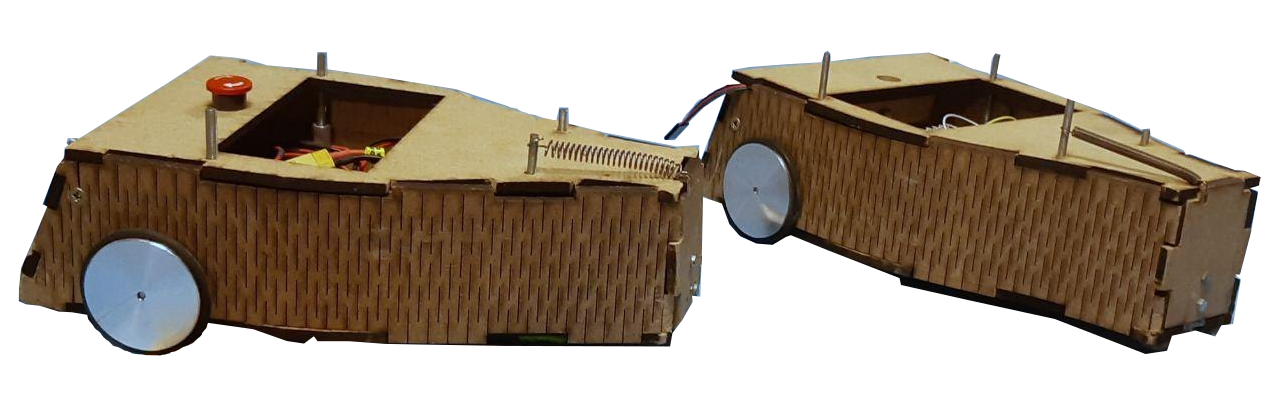
\includegraphics[scale=0.45]{brenda.png}
  \end{figure}

\begin{multicols}{2}
  \begin{figure}[H]
    \center
    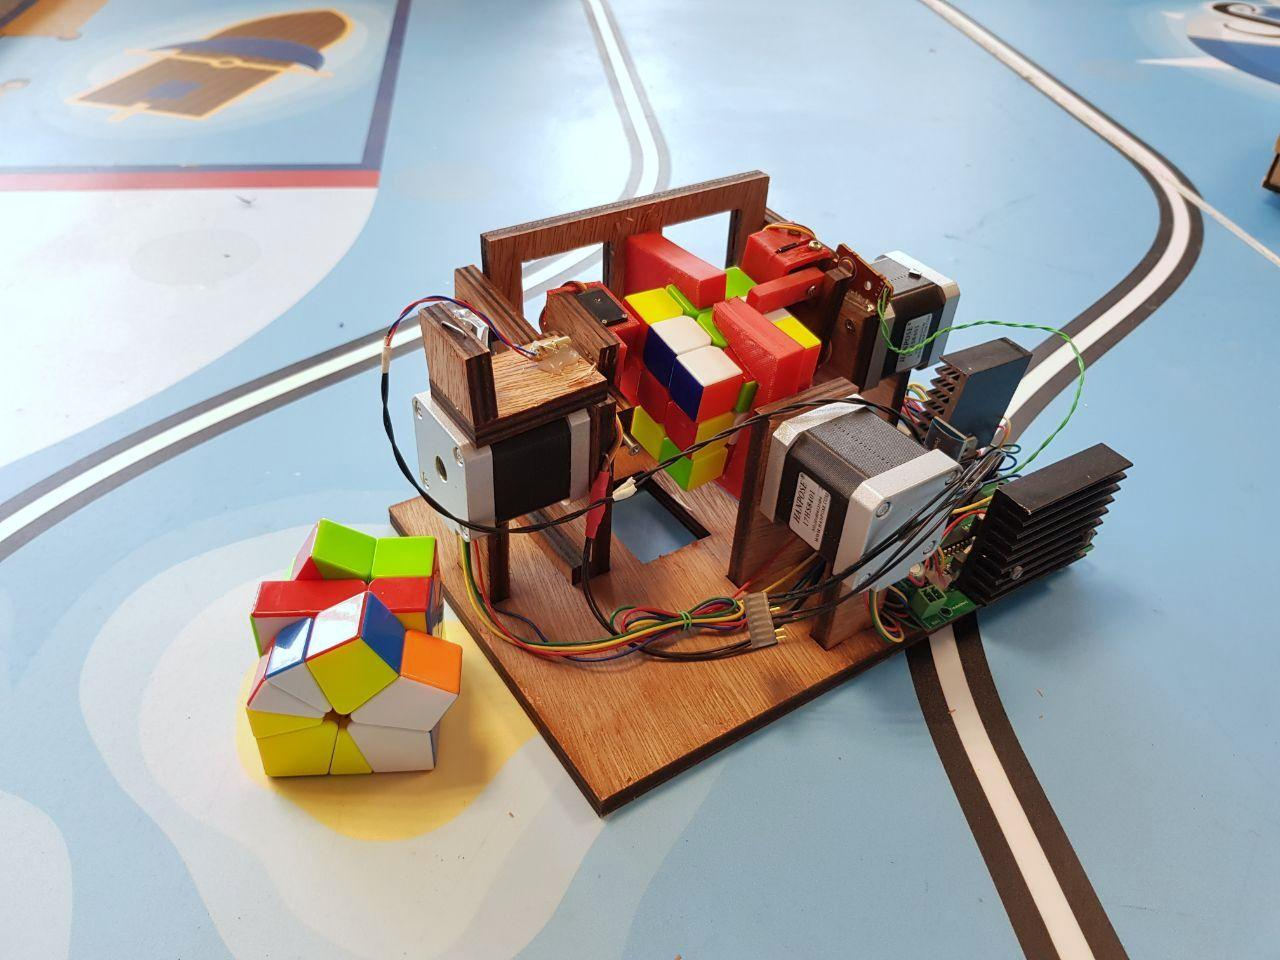
\includegraphics[scale=0.2]{rubix_cube.jpg}
  \end{figure}
  \columnbreak
  \begin{figure}[H]
    \center
    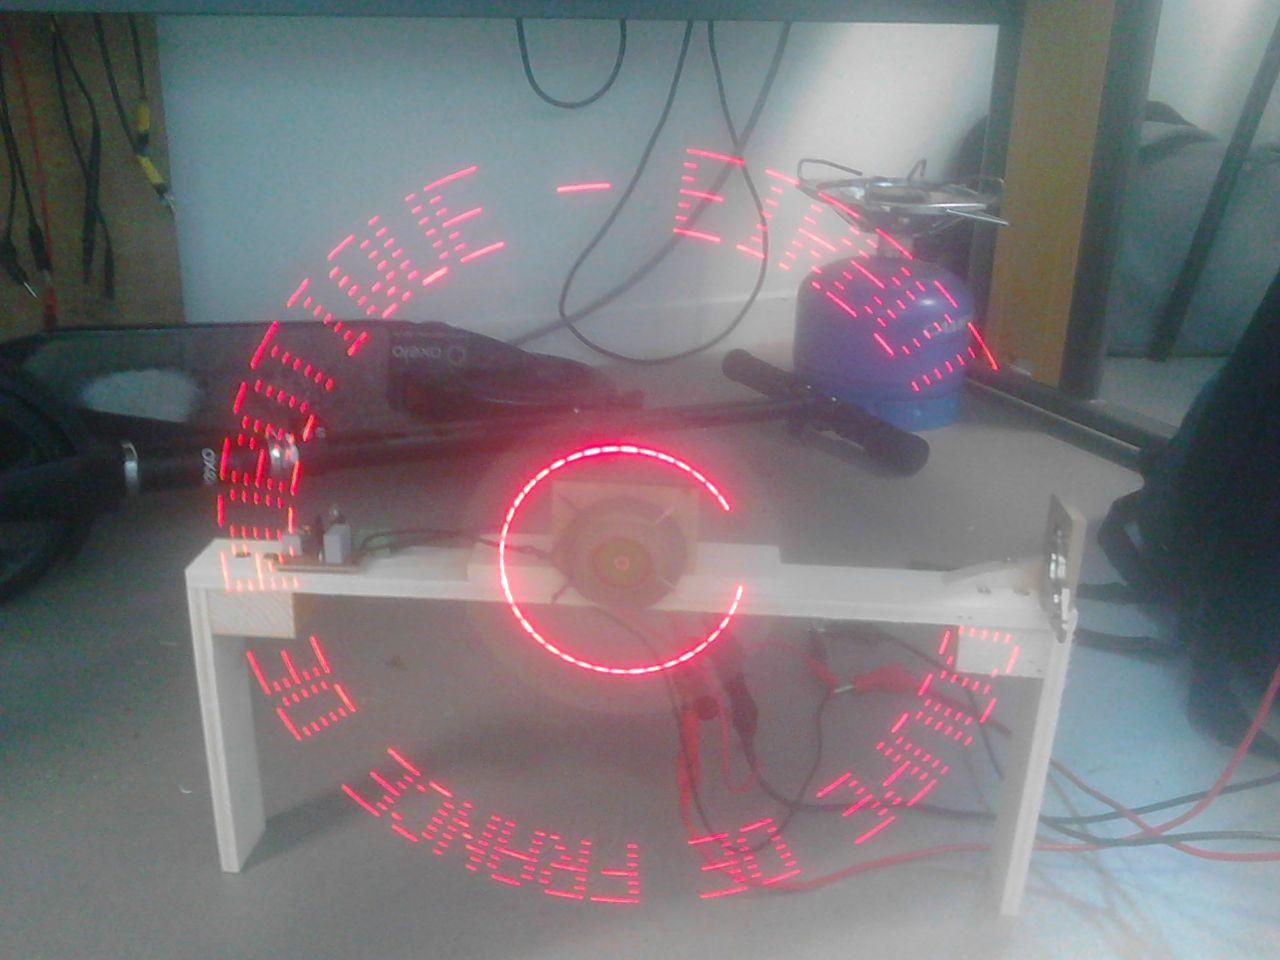
\includegraphics[scale=0.2]{tourne.jpg}
  \end{figure}
\end{multicols}

\newpage
\end{spacing}
\end{document}
%%Brouillon du mail
%%
%%Bonjour,
%%Suite à notre discussion à l'afterwork Cdiscount organisé par AEI, je vous
%%envoie la plaquette de notre association et un dossier descriptif de nos
%%projets.
%%
%%
%
